\documentclass[11pt]{article}
\usepackage[margin=1in]{geometry}
\usepackage{amsmath,amssymb}
\usepackage{graphicx}
\usepackage{tikz}
\usetikzlibrary{calc}
\usepackage{pgfplots}
\pgfplotsset{compat=1.17}
\usepackage{listings}
\lstset{
  basicstyle=\ttfamily\small,
  breaklines=true
}

\title{Comprehensive Review: Random Forests}
\author{Master's Level Data Science}
\date{}

\begin{document}
\maketitle
\tableofcontents
\bigskip

\section{Introduction}
This review synthesizes the lecture slides (\texttt{ensemble-4.pdf}) and the audio transcript (\texttt{RandomForests.txt}) on random forests. We cover motivation, the random forest algorithm, illustrative diagrams, a worked example, empirical results on the Covertype dataset, practical guidelines, and future extensions.

\section{Motivation: From Tree to Forest}
Decision trees are expressive but prone to overfitting beyond a certain size. Boosting mitigates this by sequentially reweighting examples, but it is inherently sequential and cannot be parallelized efficiently. Random forests address both issues by building many trees in parallel with injected randomness to ensure diversity and then aggregating via majority vote.

\section{Random Forest Algorithm}
Given a dataset $S$ of $n$ labeled points:
\begin{enumerate}
  \item \textbf{For} $t=1,\dots,T$ (in parallel):
    \begin{enumerate}
      \item Draw a \emph{bootstrap sample} $S_t$ of size $n'$ (typically $n'=n$) by sampling with replacement from $S$.
      \item Grow a decision tree $h_t$ on $S_t$:
        \begin{itemize}
          \item At each node, select a random subset of $k$ features (often $k=\sqrt{d}$ or $d/2$).
          \item Choose the best split among those $k$ features.
          \item Continue until a stopping criterion (e.g.\ max depth or purity) is met.
        \end{itemize}
    \end{enumerate}
  \item \textbf{Output} the ensemble classifier:
  \[
    H(x) \;=\;\mathop{\mathrm{majority\_vote}}\{\,h_t(x)\}_{t=1}^T.
  \]
\end{enumerate}
This parallel procedure yields diverse trees whose errors tend to be uncorrelated, reducing variance in aggregation:contentReference[oaicite:1]{index=1}.

\section{Geometric Illustration}
\begin{figure}[h]
\centering
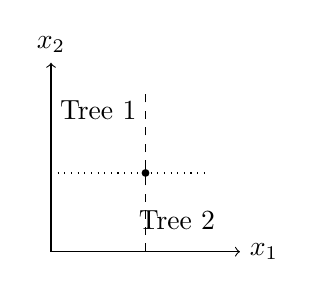
\begin{tikzpicture}[scale=2]
  % Sample of two tree partitions
  \draw[->] (0,0) -- (1.2,0) node[right] {$x_1$};
  \draw[->] (0,0) -- (0,1.2) node[above] {$x_2$};
  % Tree 1 split on x1
  \draw[dashed] (0.6,0) -- (0.6,1);
  \node at (0.3,0.9) {Tree 1};
  % Tree 2 split on x2
  \draw[dotted] (0,0.5) -- (1,0.5);
  \node at (0.8,0.2) {Tree 2};
  \draw (0.6,0.5) node[fill=black,circle,inner sep=1pt]{};
\end{tikzpicture}
\caption{Two example trees with different splits due to random feature selection.}
\end{figure}

\section{Worked Example}
We demonstrate a random forest on a synthetic binary classification dataset.

\subsection{Data Generation and Preprocessing}
\begin{lstlisting}[language=Python]
import numpy as np
from sklearn.datasets import make_classification
X, y = make_classification(
    n_samples=1000, n_features=10,
    n_informative=5, n_redundant=2,
    random_state=42
)
\end{lstlisting}

\subsection{Model Training}
\begin{lstlisting}[language=Python]
from sklearn.ensemble import RandomForestClassifier
clf = RandomForestClassifier(
    n_estimators=100,
    max_features='sqrt',
    max_depth=None,
    bootstrap=True,
    random_state=42
)
clf.fit(X, y)
\end{lstlisting}

\subsection{Model Evaluation}
\begin{lstlisting}[language=Python]
from sklearn.model_selection import cross_val_score
scores = cross_val_score(clf, X, y, cv=5, scoring='accuracy')
print("CV accuracy: %.2f +/- %.2f" % (scores.mean(), scores.std()))
\end{lstlisting}

\section{Empirical Results: Covertype Data}
On the Covertype dataset (49{,}514 train / 445{,}627 test), reported errors are:contentReference[oaicite:2]{index=2}:
\begin{itemize}
  \item Single decision tree (depth 20): test error 12.6\%.
  \item Boosted trees (10 trees, depth 20): test error 8.7\%.
  \item Random forest (10 trees, 50\% features, depth 40): test error 8.8\%.
\end{itemize}

\section{Interpretation \& Guidelines}
\begin{itemize}
  \item \textbf{Variance Reduction}: Aggregating uncorrelated trees lowers variance without increasing bias.
  \item \textbf{Feature Subsampling}: Random feature selection ensures diversity and prevents dominant features from being used in all trees.
  \item \textbf{Parallelism}: Trees can be trained in parallel, speeding up training.
  \item \textbf{Hyperparameters}: Tune $T$, $k$ (features per split), $n'$ (bootstrap size), and tree depth via cross-validation.
\end{itemize}

\section{Future Directions / Extensions}
\begin{itemize}
  \item \textbf{Out-of-Bag Error}: Use OOB samples to estimate generalization error without a separate validation set.
  \item \textbf{Feature Importance}: Compute importance scores via permutation or mean decrease in impurity.
  \item \textbf{Extremely Randomized Trees}: Use random thresholds in addition to random features.
  \item \textbf{Hybrid Ensembles}: Combine random forests with boosting or other learners for enhanced performance.
\end{itemize}

\end{document}
